% Latex template: mahmoud.s.fahmy@students.kasralainy.edu.eg
% For more details: https://www.sharelatex.com/learn/Beamer

\documentclass{beamer}					% Document class

\usepackage[english]{babel}				% Set language
\usepackage[utf8x]{inputenc}			% Set encoding

\mode<presentation>						% Set options
{
  \usetheme{default}					% Set theme
  \usecolortheme{default} 				% Set colors
  \usefonttheme{default}  				% Set font theme
  \setbeamertemplate{caption}[numbered]	% Set caption to be numbered
}

% Uncomment this to have the outline at the beginning of each section highlighted.
%\AtBeginSection[]
%{
%  \begin{frame}{Outline}
%    \tableofcontents[currentsection]
%  \end{frame}
%}

\usepackage{graphicx}					% For including figures
\usepackage{booktabs}					% For table rules
\usepackage{hyperref}					% For cross-referencing
\usepackage{subcaption}  % 記得加在 preamble
\usepackage{multicol}

\title{The Chi-squared Test of Independence}	% Presentation title
\author{Shao-Yu Wang}								% Presentation author
\institute{Department of Agronomy, National Taiwan University}					% Author affiliation
\date{\today}									% Today's date	

\begin{document}

% Title page
% This page includes the informations defined earlier including title, author/s, affiliation/s and the date
\begin{frame}
  \titlepage
\end{frame}

% Outline
% This page includes the outline (Table of content) of the presentation. All sections and subsections will appear in the outline by default.
\begin{frame}{Outline}
  \tableofcontents
\end{frame}

% The following is the most frequently used slide types in beamer
% The slide structure is as follows:
%
%\begin{frame}{<slide-title>}
%	<content>
%\end{frame}

\section{Introduction}


\begin{frame}{Introduction}
    
    Is the age of the driver related to traffic violations?
    
    \begin{figure}[H]
        \begin{minipage}[c]{.45\textwidth}
            \centering
            
\includegraphics[width=.8\textwidth]{figures/young-driving-a-car-vector.jpg}
            
            \vspace{0.5em}
            
            
\includegraphics[width=.8\textwidth]{figures/old-man-driving-vintage-car-with-old-man-driving-it_497046-2966 (1).png}
        \end{minipage}
        \hfill
        \begin{minipage}[c]{.45\textwidth}
            \centering
            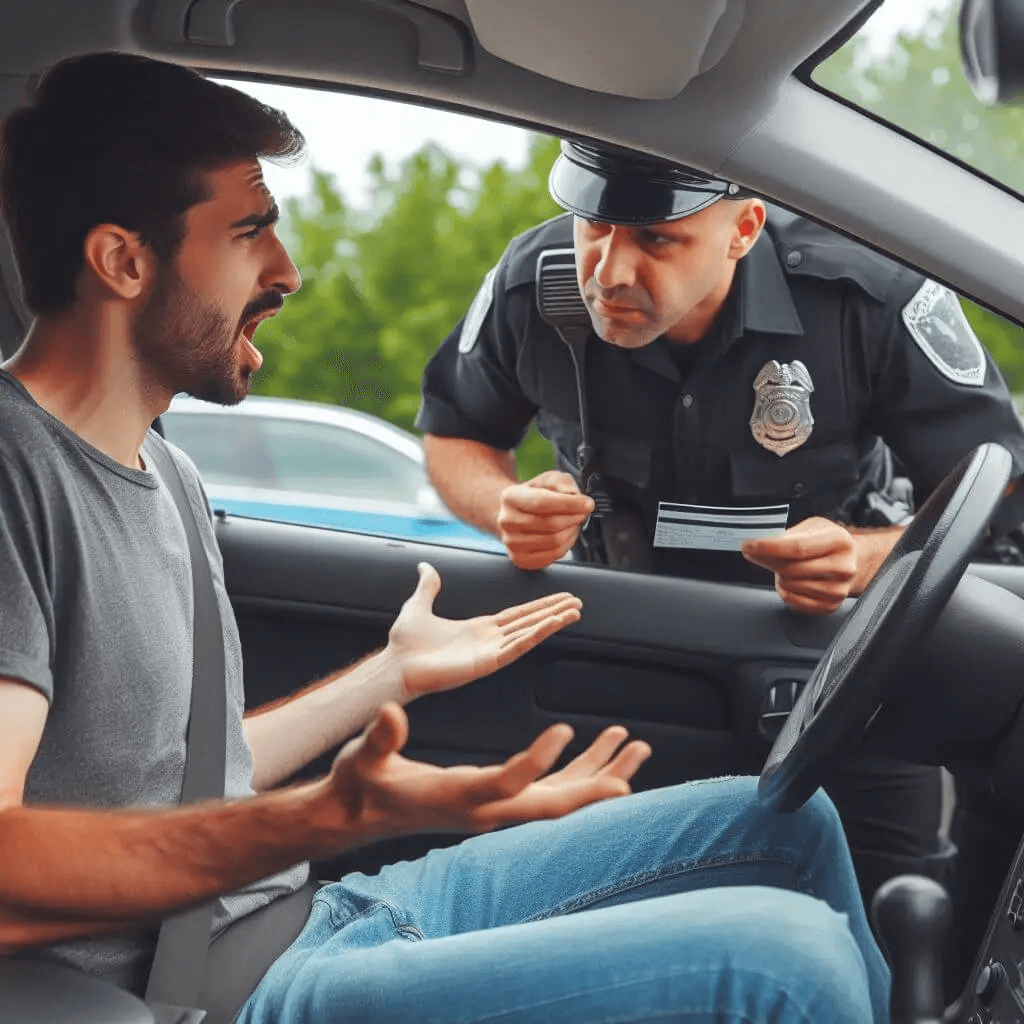
\includegraphics[width=\textwidth]{figures/feature-image-queens.png}
        \end{minipage}
    \end{figure}
\end{frame}

\begin{frame}{Why Do We Use the Chi-squared Test?}

\small
\begin{columns}[T,onlytextwidth]

\column{0.48\textwidth}
\begin{block}{Categorical Variables}
\begin{itemize}
    \item Data are \textbf{categories}
    \item Summarized as \textbf{counts / frequencies}
    \item Examples:
    \begin{itemize}
        \item Gender
        \item Age group
        \item Disease status
    \end{itemize}
\end{itemize}
\end{block}

\column{0.48\textwidth}
\begin{block}{Continuous Variables}
\begin{itemize}
    \item Data are \textbf{numerical}
    \item Summarized by \textbf{means / variances}
    \item Examples:
    \begin{itemize}
        \item Height
        \item Weight
        \item Blood pressure
    \end{itemize}
\end{itemize}
\end{block}

\end{columns}

\vspace{0.6em}
\begin{alertblock}{Key Idea}
Continuous data → t-test / ANOVA \\
Categorical data → \textbf{Chi-squared test}
\end{alertblock}

\end{frame}


\begin{frame}{Types of Chi-squared Tests}

\small
There are three main types of Chi-squared tests:
    
\vspace{0.8em}
\begin{itemize}
    \item \textbf{Test of Independence} ← Today's focus \\
    \hspace{1em} Tests whether {two categorical variables are associated}
    
    \vspace{0.6em}
    \item \textbf{Goodness-of-Fit Test} \\
    \hspace{1em} Tests whether {observed frequencies match a specified distribution}
    
    \vspace{0.6em}
    \item \textbf{Test of Homogeneity} \\
    \hspace{1em} Tests whether {multiple populations share the same distribution}
\end{itemize}
    
\vspace{0.8em}
\begin{alertblock}{Key Point}
What they test is quite different, but the process is very similar.
\end{alertblock}

\end{frame}

\begin{frame}{Test of Independence}
    \textbf{Purpose:} Test whether two categorical variables are independent
    
    \vspace{1em}
    \textbf{Example:}
    \begin{itemize}
        \item Variable 1: Driver age ($\le 30$ vs $> 30$)
        \item Variable 2: Number of traffic violations (0, 1-2, $>2$)
    \end{itemize}
    
    \vspace{1em}
    \textbf{Question:} Are these two variables independent?
\end{frame}

\begin{frame}{Contingency Table}
    \begin{table}[H]
\centering
\caption{Contingency Table of Driver Age and Traffic Violations}
\label{tab:table1}
\begin{tabular}{@{}l|ccc|c@{}}
\toprule
 & \multicolumn{3}{c|}{\textbf{Number of Violations}} & \\
\cmidrule{2-4}
\textbf{Age Group} & \textbf{0} & \textbf{1-2} & \textbf{$>$2} & \textbf{Total} \\ 
\midrule
30 $\le$ & 18 & 76 & 39 & 133 \\
$>$ 30 & 32 & 54 & 26 & 112 \\
\midrule
\textbf{Total} & 50 & 130 & 65 & 245 \\ 
\bottomrule
\end{tabular}
\end{table}
    
    \vspace{0.5em}
    \begin{itemize}
        \item Rows: Age groups
        \item Columns: Number of violations
        \item Cells: Observed frequencies
    \end{itemize}
\end{frame}

\section{Chi-squared Test Procedure}

\begin{frame}{Step 1: Set Up Hypotheses}
    \textbf{Hypotheses:}
    $$
    \begin{cases}
    H_0: \text{A and B are independent} \\
    H_1: \text{A and B are not independent}
    \end{cases}
    $$
    
    \vspace{1em}
    \textbf{Significance level:} $\alpha = 0.05$
\end{frame}

\begin{frame}{Step 2: Test Statistic}
    \textbf{Formula:}
    $$
    \chi^2 = \sum_{i,j} \frac{(O_{ij} - E_{ij})^2}{E_{ij}}
    $$
    
    where:
    \begin{itemize}
        \item $O_{ij}$ = Observed frequency
        \item $E_{ij}$ = Expected frequency (calculated assuming $H_0$ is true)
    \end{itemize}
    
    \vspace{0.5em}
    \textbf{Degrees of freedom:} $df = (r-1)(c-1) $\\
    where:
    \begin{itemize}
        \item $r$ = Number of raws
        \item $c$ = Number of columns
    \end{itemize}
    \vspace{0.5em}
    \begin{alertblock}{Notes}
    Every $E_{ij}$ should be $\geq 5$; otherwise, you should combine categories until all expected frequencies are $\geq 5$.
    \end{alertblock}
\end{frame}

\begin{frame}{Step 3 \& 4: Expected Frequencies \& Rejection Region}
    \textbf{Formula:}
    $$
    E_{ij} = \frac{(\text{Row}_i \text{ total}) \times (\text{Column}_j \text{ total})}{\text{Grand total}} = \frac{R_i \times C_j}{n}$
    $$
    

    \textbf{Rejection Region}
$$
RR = \left\{ \chi^2 : \chi^2 \ge \chi^2_{\alpha, df} \right\}
$$
\begin{figure}
        \centering
        
\includegraphics[width=0.7\textwidth]{right-tailed-chi-square-test.png}
    \end{figure}
\end{frame}


\section{Worked Example}
\begin{frame}{Worked Example}
    We want to test whether age and traffic violations are independent.
    \begin{table}[H]
\centering
\caption{Contingency Table of Driver Age and Traffic Violations}
\label{tab:table1}
\begin{tabular}{@{}l|ccc|c@{}}
\toprule
 & \multicolumn{3}{c|}{\textbf{Number of Violations}} & \\
\cmidrule{2-4}
\textbf{Age Group} & \textbf{0} & \textbf{1-2} & \textbf{$>$2} & \textbf{Total} \\ 
\midrule
30 $\le$ & 18 & 76 & 39 & $R_{1}=133$\\
$>$ 30 & 32 & 54 & 26 & $R_{2}=112$\\
\midrule
\textbf{Total} & $C_{1} = 50$ & $C_{2}=130$ & $C_{3}=65$ & $n =$ 245 \\ 
\bottomrule
\end{tabular}
\end{table}

\end{frame}

\begin{frame}{Hypotheses \& Calculate Expected Frequencies}
    \textbf{Hypotheses:}
    $$
    \begin{cases}
    H_0: \text{Driver's Age and Traffic Violation are independent} \\
    H_1: \text{Driver's Age and Traffic Violation are not independent}
    \end{cases}
    $$
\textbf{Formula:}
$$
E_{ij} = \frac{R_i \times C_j}{n}
$$
\vspace{0.5em}
    \small
    \begin{columns}[T]
        \column{.5\textwidth}
        \text{Row 1 ($\le 30$):}
        \begin{align*}
        E_{11} &= \frac{133\times50}{245} = 27.14 \\[0.8em]
        E_{12} &= \frac{133\times130}{245} = 70.57 \\[0.8em]
        E_{13} &= \frac{133\times65}{245} = 35.29
        \end{align*}
        
        \column{.5\textwidth}
        \text{Row 2 ($> 30$):}
        \begin{align*}
        E_{21} &= \frac{112\times50}{245} = 22.86 \\[0.8em]
        E_{22} &= \frac{112\times130}{245} = 59.43 \\[0.8em]
        E_{23} &= \frac{112\times65}{245} = 29.71
        \end{align*}
    \end{columns}
    

\end{frame}

\begin{frame}{Observed vs Expected Frequencies}
    \begin{table}[H]
\centering
\caption{Contingency Table of Driver Age and Traffic Violations}
\label{tab:table1}
\begin{tabular}{@{}l|ccc|c@{}}
\toprule
 & \multicolumn{3}{c|}{\textbf{Number of Violations}} & \\
\cmidrule{2-4}
\textbf{Age Group} & \textbf{0} & \textbf{1-2} & \textbf{$>$2} & \textbf{Total} \\ 
\midrule
30 $\le$ & 18(27.14) & 76(70.57) & 39(35.29) & 133 $R_{1}$\\
$>$ 30 & 32(22.86) & 54(59.43) & 26(29.71) & 112 $R_{2}$\\
\midrule
\textbf{Total} & 50 & 130 & 65 & $n =$ 245 \\ 
\ & $C_{1}$ & $C_{2}$ & $C_{3}$ &  \\ 
\bottomrule
\end{tabular}
\end{table}
    
    \vspace{0.5em}
    Notice the differences between observed and expected values
\end{frame}

\begin{frame}{Calculate Test Statistic}
    \small
    \begin{align*}
    \chi^2 &= \sum\limits_{i=1}^2 \sum\limits_{j=1}^3 \frac{(O_{ij} - E_{ij})^2}{E_{ij}} \\[0.5em]
    &= \frac{(18 - 27.14)^2}{27.14} + \frac{(76 - 70.57)^2}{70.57} + \frac{(39 - 35.29)^2}{35.29} \\[0.3em]
    &\quad + \frac{(32 - 22.86)^2}{22.86} + \frac{(54 - 59.43)^2}{59.43} + \frac{(26 - 29.71)^2}{29.71} \\[0.5em]
    &= 3.08 + 0.42 + 0.39 + 3.65 + 0.50 + 0.46 \\[0.3em]
    &= 8.50
    \end{align*}
\end{frame}

\begin{frame}{Make Decision}
    \textbf{Test Statistic:} $\chi^2 = 8.50$
    
    \textbf{Degrees of Freedom:} $df = (r-1)(c-1)=(2-1)(3-1)=2$
    
    \textbf{Critical Value:} $\chi^2_{0.05, 2} = 5.991$
    
    \vspace{1em}
    
    \begin{block}{Decision}
    Since $\chi^2 = 8.50 > 5.991$, we \textbf{reject $H_0$}
    \end{block}
    
    \vspace{0.5em}
    
    \begin{alertblock}{Conclusion}
    Driver age and traffic violations are \textbf{NOT independent}.
    
    There is a significant relationship between age and violations.
    \end{alertblock}
\end{frame}



\section{R Implementation}

\begin{frame}[fragile]{Step 1: Create Data Matrix}
Creating a contingency table in R

    \begin{figure}
        \centering
        
\includegraphics[width=0.9\textwidth]{dataset.png}
    \end{figure}
    Here is how the data matrix looks like
    \begin{figure}
        \centering
        
\includegraphics[width=0.3\textwidth]{截圖 2026-01-29 上午10.17.48.png}
    \end{figure}
\end{frame}

\begin{frame}[fragile]{Step 2: Run Chi-squared Test}
    \textbf{Function:} \texttt{chisq.test(data)}
    
    \begin{figure}
        \centering
        
\includegraphics[width=0.9\textwidth]{result.png}
    \end{figure}
    
    \vspace{0.5em}
    \begin{itemize}
        \item $\chi^2 = 8.5056$
        \item $p$-value $= 0.0142 < 0.05$ → Reject $H_0$
    \end{itemize}
\end{frame}

\begin{frame}{Interpreting R Output}
    \textbf{Key Information:}
    \begin{itemize}
        \item \textbf{X-squared:} Test statistic value
        \item \textbf{df:} Degrees of freedom
        \item \textbf{p-value:} Probability of observing this result if $H_0$ is true
    \end{itemize}
    
    \vspace{1em}
    
    \begin{block}{Decision Rule}
    If $p$-value $< \alpha$ (usually 0.05), reject $H_0$
    \end{block}
\end{frame}

\section{Summary}

\begin{frame}{Summary: Chi-squared Test Steps}
    \begin{enumerate}
        \item Collect data → Contingency table
        \item Set up hypotheses ($H_0$: independent)
        \item Calculate expected frequencies
        \item Compute $\chi^2$ statistic
        \item Compare with critical value or check $p$-value
        \item Make decision and conclude
    \end{enumerate}
    
    \vspace{1em}
    
    \begin{block}{R Implementation}
    One simple command: \texttt{chisq.test(data)}
    \end{block}
\end{frame}

\begin{frame}{}    
    \begin{center}
    \Large Thank you for your attention!
    \end{center}
\end{frame}
\end{document}
